\documentclass[]{article}
\usepackage{jcappub} % for details on the use of the package, please
\newcommand{\mnras}{{\em Mon. Not. Roy. Astron. Soc. }}
\newcommand{\apjl}{{\em Astrophys. J. Let. }}
\newcommand{\apjs}{ApJS}
\newcommand{\apj}{ApJ}
\newcommand{\jcap}{JCAP}
\newcommand{\physrep}{{\em Phys. Rept. }}
\newcommand{\aap}{{\em Astron. Astrophys. }}
\newcommand{\aj}{AJ }
\newcommand{\pasp}{PASP}
\newcommand{\pasj}{PASJ}
\def\prd{{\em Phys. Rev. }{\bf D }}
\def\prl{{\em Phys. Rev. }{\bf L }}
\def\pr{{Phys.\ Rev.\ }}
\def\astropart{{Astro-particle Phys.~}}
\def\rvmp{{Rev.\ Mod.\ Phys.\ }}
\newcommand{\lyaf}{Ly$\alpha$ forest }                     % see the JCAP-author-manual
\newcommand{\lya}{Ly$\alpha$}
%opening
\title{Parametrisation of a Lyman-$\alpha$ forest emulator.}

\author[a]{Chris Pedersen}
\affiliation[a]{Department of Physics and Astronomy, University College London, Gower Street, London, United Kingdom}
\emailAdd{chrisp@star.ucl.ac.uk}

\abstract{Set of notes discussing parametrisations of an emulator for cosmology from 
the Lyman-$\alpha$ forest. This is meant primarily as an intituive introduction to
our parametrisation rather than a discussion of the technical details,
some of which will be included in Appendix C.}
\begin{document}
\maketitle

\section{Introduction}
Constraining parameters of a cosmological model requires a large number of theoretical 
predictions to compare to observational data. In the case of the Lyman-$\alpha$ (\lya) 
forest, generating these theoretical predictions are computationally expensive which makes a 
brute-force approach unfeasible. Interpolation schemes have therefore been proposed where 
theoretical predictions are made at certain points in parameter space, and these then are 
used to infer the observable quantities for an arbitrary model.
Our fundamental assumption is that the flux power spectrum of the \lyaf at any given 
redshift is determined by the amplitude and shape of the linear matter power spectrum, 
and the state of the intergalactic medium (IGM). Under this assumption the standard 
$\Lambda$CDM parameters become impractical for \lyaf analysis due to parameter 
degeneracies and difficulties in parametrising the state of the IGM. Therefore instead of 
constraining the cosmological parameters of the $\Lambda$CDM model directly, we intend to 
constrain the amplitude and slope of the linear power spectrum and its evolution with 
redshift, while marginalising over the IGM parameters (an approach that was taken in ref 
\cite{McDonald2005}). For our purposes we then need to introduce three different 
parameter spaces:


\begin{itemize}
    \item an \textit{emulator space} where we train a Gaussian process to provide a 
    predicted 1D flux power spectrum for a given set of parameters that we believe to be 
    closest to the data,
    \item a \textit{likelihood space} which describes the amplitude and redshift 
    evolution of the linear matter power spectrum and the IGM parameters, which is where 
    we run our sampler,
    \item a \textit{simulation space}, which consists of the parameters which we can 
    input into MP-Gadget simulations (these are mostly $\Lambda$CDM parameters with some 
    parameters which affect the IGM history)
\end{itemize}

\section{Parameter spaces}
\subsection{Emulator space}
Due to the fact that the universe is very close to Einstein-de-Sitter in the relevant 
redshfit range $(5>z>2)$, the growth factor, $D(z)$ and the evolution of the Hubble 
expansion rate, $H(z)$, are close to independent of cosmology. The \lyaf is also 
sensitive to only a small range of length scales within this redshift range 
(approximately $0.1 \mathrm{Mpc}^{-1} < k < 10 \mathrm{Mpc}^{-1}$), meaning that the large 
scale shape of the power spectrum also has no influence on the \lyaf. Given this, the 
effect of changing various $\Lambda$CDM parameters on the 1 dimensional flux power 
spectrum (P1D) of the \lyaf are highly degenerate with one another. Many of these effects 
will also arise through changing the thermal history of the IGM, which is something one 
would ideally decouple from cosmology and marginalise over. Instead we describe each 
measured P1D by a set of parameters which describe the linear power spectrum and the 
thermal state of the IGM. We use the following parameters:

\begin{itemize}
    \item $\Delta^2_p$: the amplitude of the matter power spectrum at $k=0.7 \mathrm{Mpc}^
    {-1}$. This scale is chosen as it is both a linear mode, and a length scale which is 
    measured well in the P1D of the \lyaf.
    \item $n_p$: the slope of the matter power spectrum around $k=0.7 \mathrm{Mpc}^{-1}$,
    \item $\alpha_p$: the running of the matter power spectrum around the same pivot 
    scale.
    \item $\langle F\rangle$: the mean flux measured along the lines of sight in
     a given simulation snapshot. 
    This property is affected mainly by the intensity of the UV background and the 
    recombination rate, as well as the amount of clustering.
    \item $\sigma_T$: the thermal broadening scale (in velocity units). This quantifies 
    the effect of the instantaneous gas pressure on smoothing the small scale flux power 
    by measuring the temperature at mean density.
    \item $\gamma$: the relation between gas temperature and density is well
    approximated by a power law, where the exponent to this power law is $\gamma-1$.
    \item $k_F$: the pressure smoothing scale. While the flux power along the line of 
    sight is dependent on the instantaneous gas pressure due to Doppler smoothing, there 
    is also a history-dependent smoothing scale caused by gas pressure\cite{Hui1997}\cite{Gnedin1998}.
\end{itemize}

\noindent We define our emulator parameter space as $\Phi=\{ \Delta^2_p,n_p,\alpha_p,\langle F\rangle,\sigma_T,\gamma,k_F \}$, and we refer to each P1D with an associated 
$\Phi$ as a \textit{model}. Note that we do not include redshift as a parameter, as we 
propose that two flux power spectra at different redshifts but with the same $\Phi$ would 
have indistinguishable flux power spectra at our current precision. This parametrisation 
can be split into two groups - parameters that describe the linear power, and parameters 
that describe the state of the IGM, which we will consider nuisance parameters. Recent 
observational constraints on these IGM properties are available in \cite{Walther2018} and 
can be used to motivate our priors. We note that one can modify the particle properties 
of the simulation data in postprocessing to explore a wider range of $\langle F\rangle$ 
and $\sigma_T$ models without running extra simulations. Since each model is decoupled 
now from $\Lambda$CDM parameters and redshift, models from different simulations can be 
pooled into one training set for the interpolation algorithm.

\subsection{Likelihood space}
The likelihood parameter space is where we run our sampler, and these are the parameters 
for which we ultimately get constraints. In the case of the nuisance parameters, these
parameters are simply power laws in the emulator parameters of the form:

\begin{equation}
    f(z)=A\bigg(\frac{1+z}{1+z_\star}\bigg)^B
\end{equation}

\noindent where we swap $f(z)$ for the relevant IGM parameter, with the pivot 
redshift $z_\star=3$. We denote the likelihood parameters as $\Theta=\{ \Delta^2_\star, f_\star, n_\star, \alpha_\star, \tau_0, \tau_1, T_1, T_2, T_3, \gamma_0, \gamma_1, k_{F0}, k_{F1} \}$, where:

\begin{itemize}
    \item $\Delta^2_\star$: which describes the amplitude of the linear power spectrum at 
    the pivot scale and redshift.
    \item $f_\star$: the logarithmic growth rate around the pivot redshift
    \item $n_\star$: the slope of the power spectrum at the pivot scale and redshift,
    \item $\alpha_\star$: the running of the power spectrum at the pivot scale and redshift.
    \item  $\tau_0$ and $\tau_1$, which equivalently describe the amplitude and slope of $\langle F\rangle$ around $z=3$,
    \item  $T_1$, $T_2$, $T_3$ which describe the redshift evolution of the thermal 
    broadening scale, $\sigma_T$. The effect of He II reionisation on the IGM means that 
    a broken power law is required to describe the evolution of the gas temperature (see 
    Appendix B). Currently the break is fixed at $z=3.6$.
    \item $\gamma_0$, $\gamma_1$, and $k_{F0}$, $k_{F1}$ which equivalently describe the amplitude and evolution of $\gamma$ and $k_F$ with redshift.
\end{itemize}

\noindent Some experimentation will be required to determine the optimum number of 
parameters to use for each power law. The specific redshifts at which emulator calls are 
made are set by the data, and one advantage of our parametrisation is that this can be 
set arbitrarily instead of being decided in advance.

\subsection{Example: maximising a likelihood}
As an example likelihood maximisation, we consider a test case where we are only interested 
in constraining the likelihood parameters $\tau_0$ and $\tau_1$, with data redshift bins 
at $z=4,3,2$. These parameters govern the amplitude and redshift evolution of $\langle F\rangle$.
The effect of this parameter is essentially just a rescaling of the overall amplitude of the flux
power spectrum, as can be seen in the top right panel of Appendix A.
Initially $\tau_0$ and $\tau_1$ are randomly chosen from within the prior 
volume, leading to 3 emulator calls evaluating equation (2.1) at each redshift where we 
have data. The likelihood evaluation is then the sum of the log likelihoods for each 
emulator call. This is shown in Fig. 1, where the mock data is shown in solid lines.
In dashed lines we show the predicted flux power spectra for four different choices of
$\tau_0$ and $\tau_1$. In the first case (top left), we show the predicted P1D for a randomly selected
$\tau_0$ and $\tau_1$, which is clearly a poor fit to the data.


\begin{figure}[h]
    \centering
    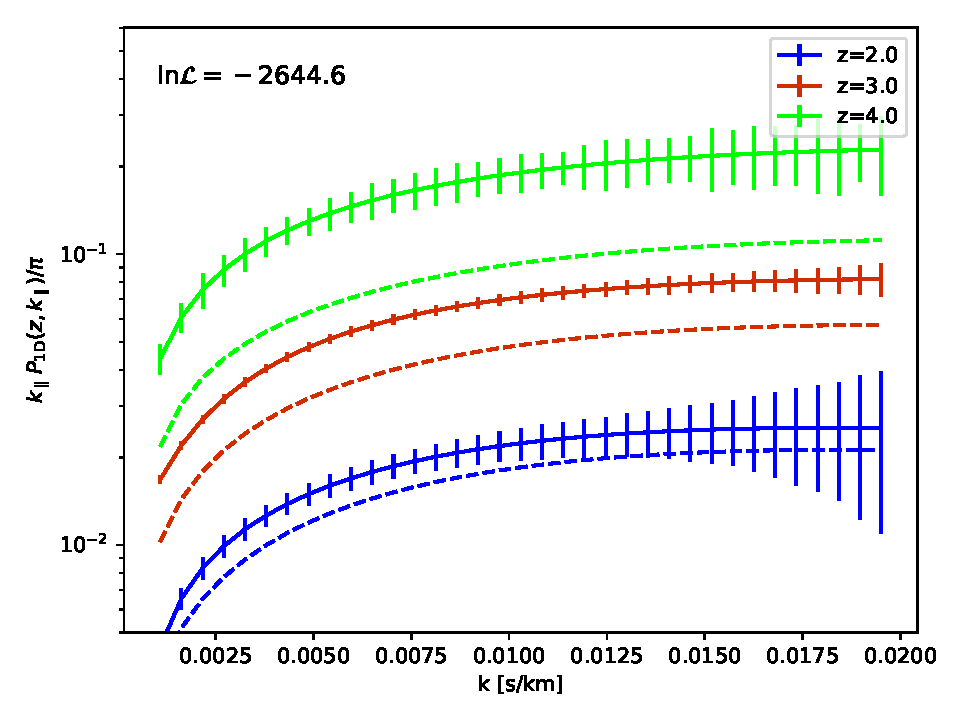
\includegraphics[scale=0.4]{Figures/random_likelihood.pdf}
    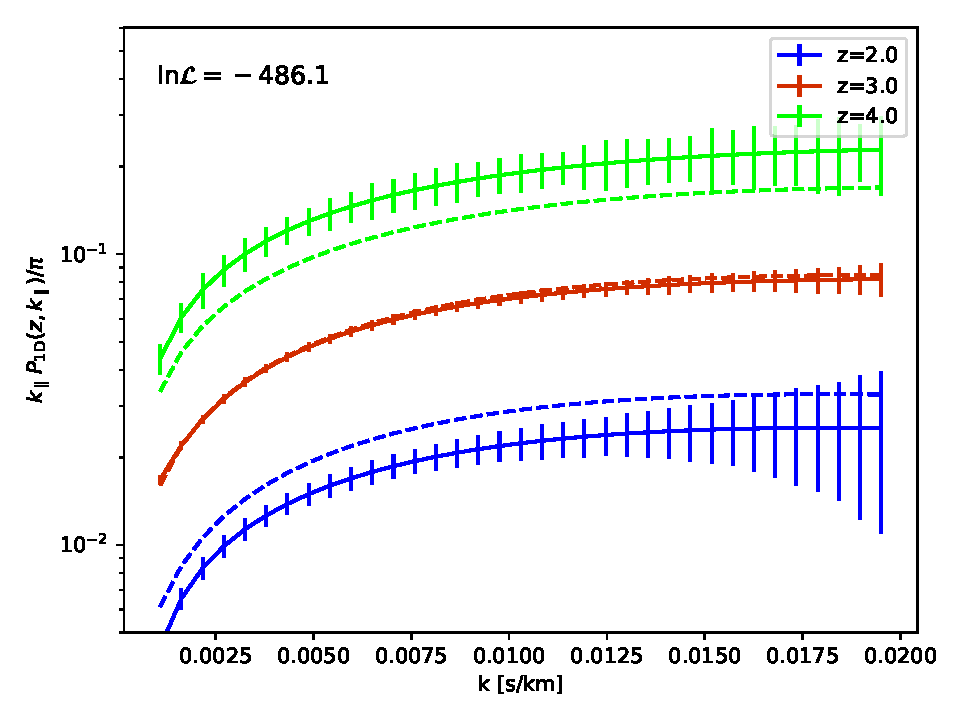
\includegraphics[scale=0.4]{Figures/amp_correct.pdf}
    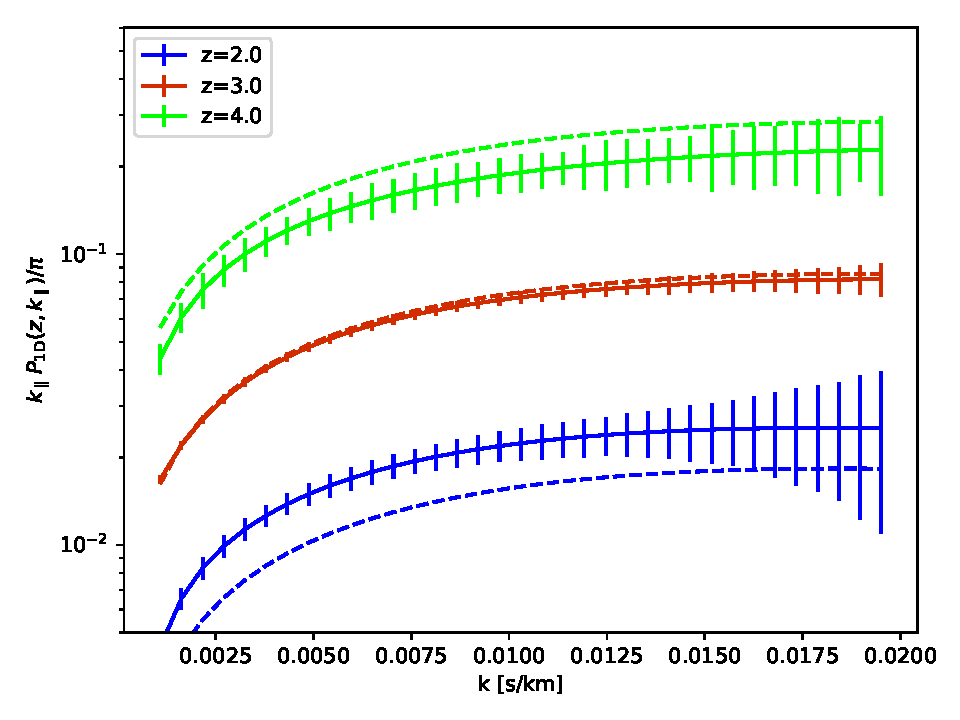
\includegraphics[scale=0.4]{Figures/growth_too_high.pdf}
    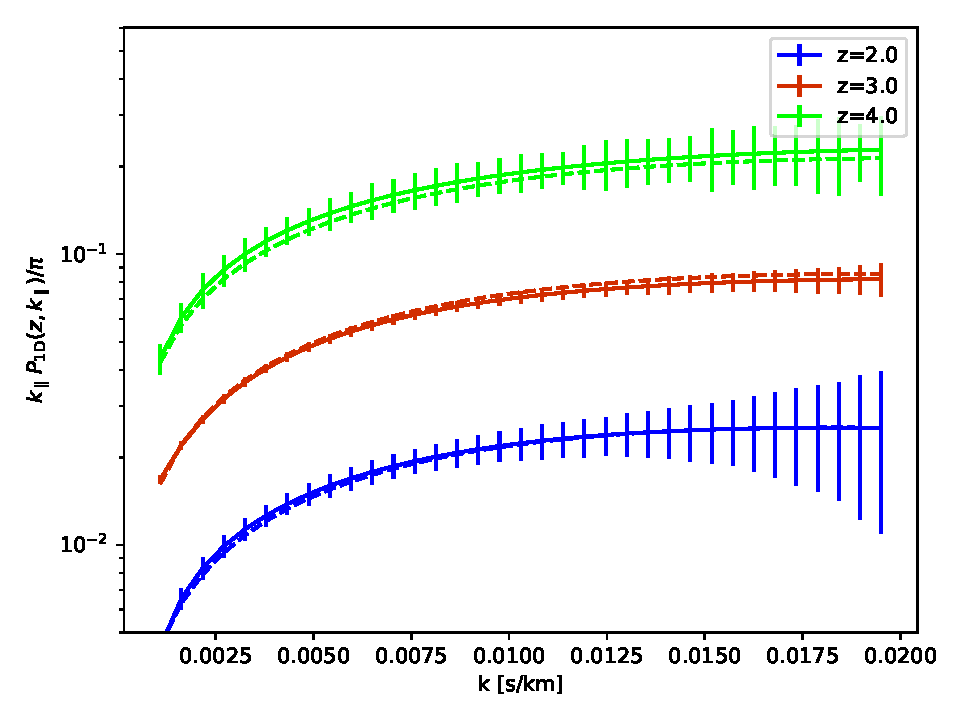
\includegraphics[scale=0.4]{Figures/goodFit.pdf}
    \caption{Predicted 1D flux power spectra (dashed) for 4 different sets of likelihood
    parameters, $\Theta$, overlaid on some mock data (solid lines with error bars) generated
    in MP-Gadget.
    The top left panel shows a randomly chosen point in likelihood space. In the top
    right we show emulator calls for likelihood parameters with the correct $\tau_0$,
    but a low $\tau_1$, resulting in insufficient redshift evolution of $\langle F\rangle$.
    In the bottom left, we show another set of emulator calls for the correct $\tau_0$
    but this time a $\tau_1$ that is too high. In the bottom right we show the emulator
    calls for the correct $\tau_0$ and $\tau_1$ which match the data well at all redshifts.}
\end{figure}

\noindent In the top right figure, we by hand fix $\tau_0$ to the correct value in the mock data, which results in the $z=3$ power spectra matching the data well.
The data at other redshifts is a poor match
however as $\tau_1$ which governs the redshift evolution is far from the correct value.
In the bottom left figure, we show emulator calls for likelihood parameters
where $\tau_0$ is still correct, however $\tau_1$ is now far too high instead of too low.
In this case there is too much evolution in the mean flux, $\langle F\rangle$, which
means the overall amplitude of the P1D changes too drastically. In the final, bottom right
panel, we show the emulator calls for the correct values of $\tau_0$ and $\tau_1$, where
there is a strong match between the emulator predictions and the data at all redshifts.
This is a particularly intuitive example because of the way in which the P1D depends
on $\langle F\rangle$, but the principle can be extended to all other parameters and
a larger number of redshift bins.

\section{Comparison with previous approaches}

\bibliographystyle{JHEP.bst}
\bibliography{refs}
\clearpage
\appendix
\section{Parameter dependence of the 1-dimensional flux power spectrum}
\begin{figure}[h]
    \centering
    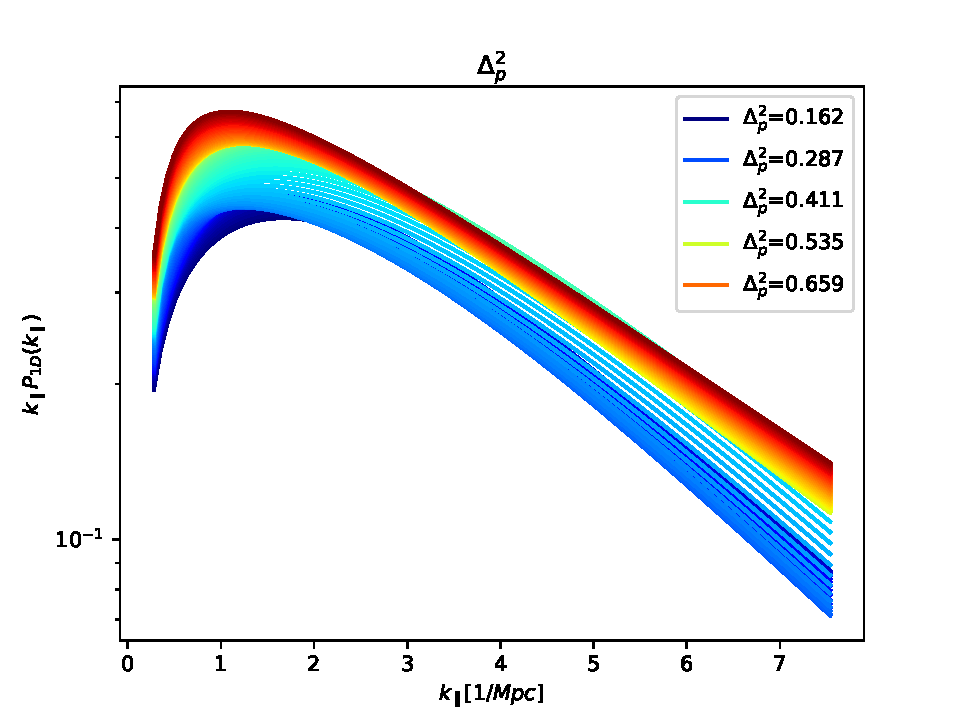
\includegraphics[scale=0.47]{Figures/256_Delta2_p.pdf}
    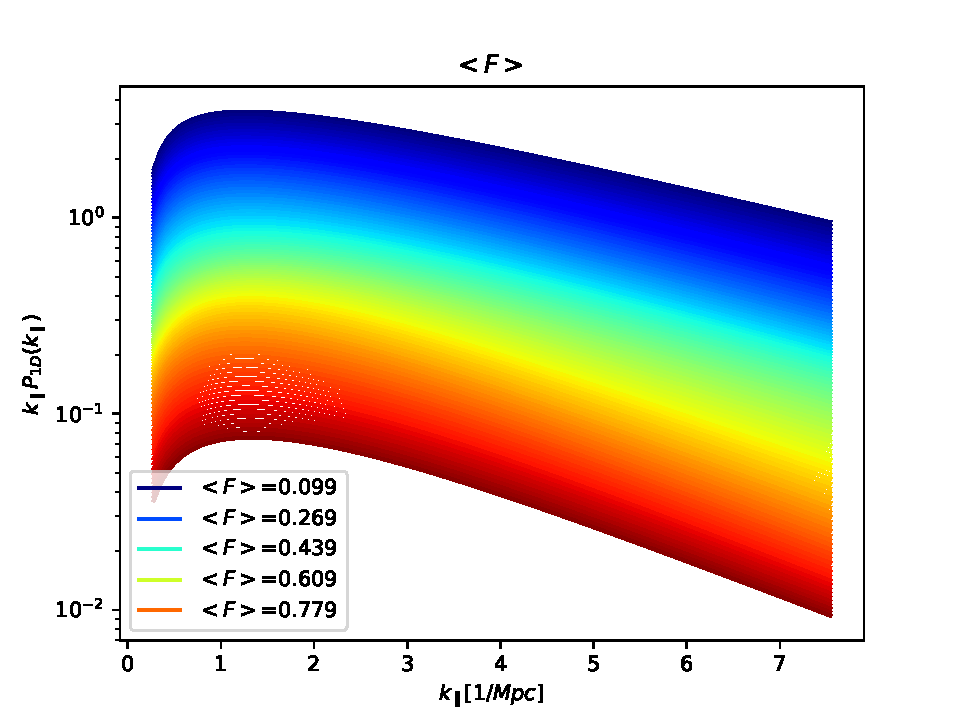
\includegraphics[scale=0.47]{Figures/256_mF.pdf}
    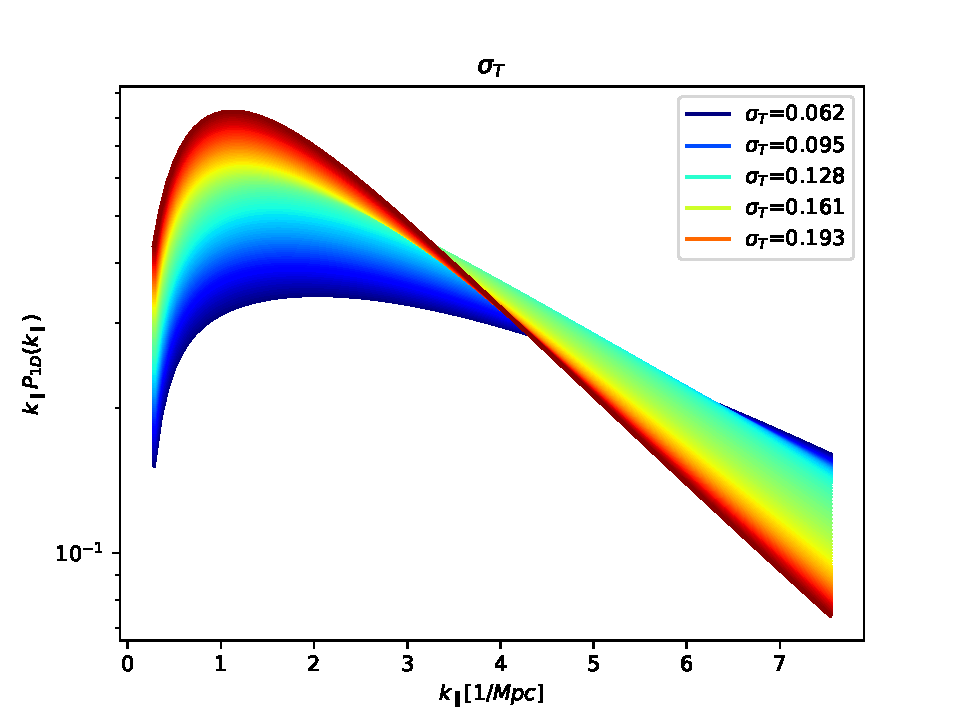
\includegraphics[scale=0.47]{Figures/256_sigT_Mpc.pdf}
    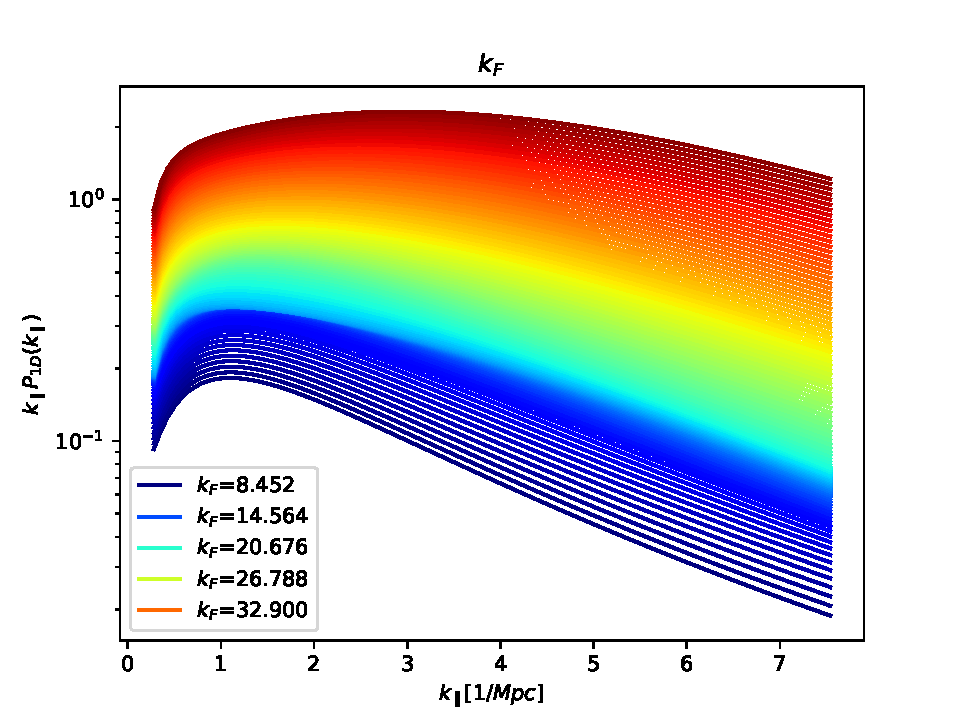
\includegraphics[scale=0.47]{Figures/256_kF_Mpc.pdf}
    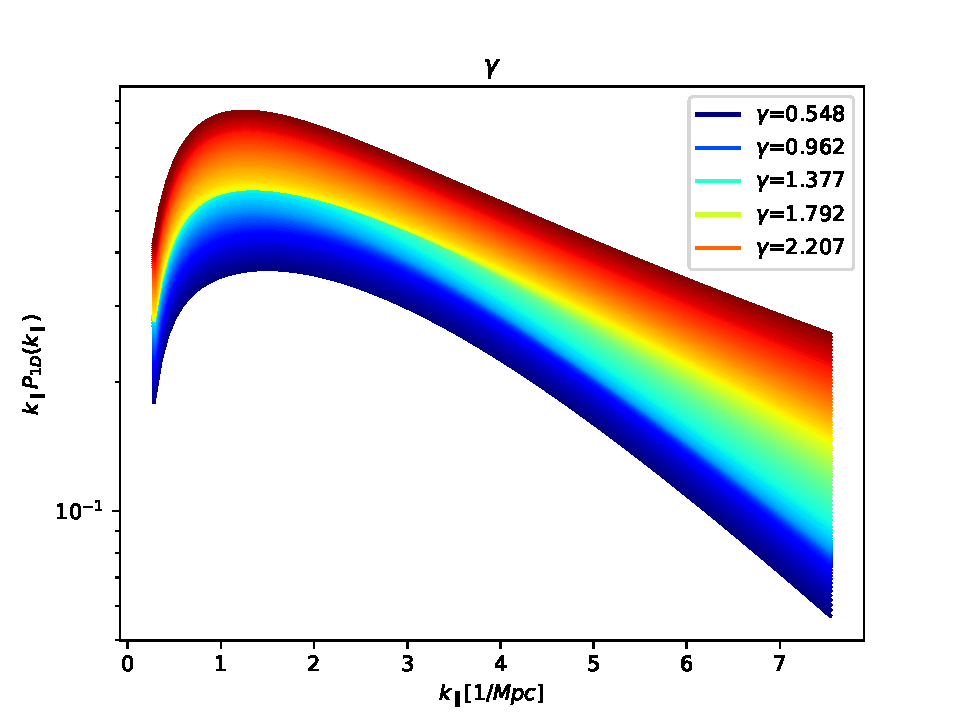
\includegraphics[scale=0.47]{Figures/256_gamma.pdf}
    \caption{Dependence of the P1D on the different emulator parameters. Predictions are 
    made using a Gaussian process emulator trained on $\sim6000$ models. NB that we have not 
    yet varied the slope ($n_p$) or running ($\alpha_p$) of the linear power spectrum in 
    our simulation suites, so do not include them here as emulated parameters.}
\end{figure}

\clearpage
\section{Redshift evolution of nuisance parameters}
\begin{figure}[h]
    \centering
    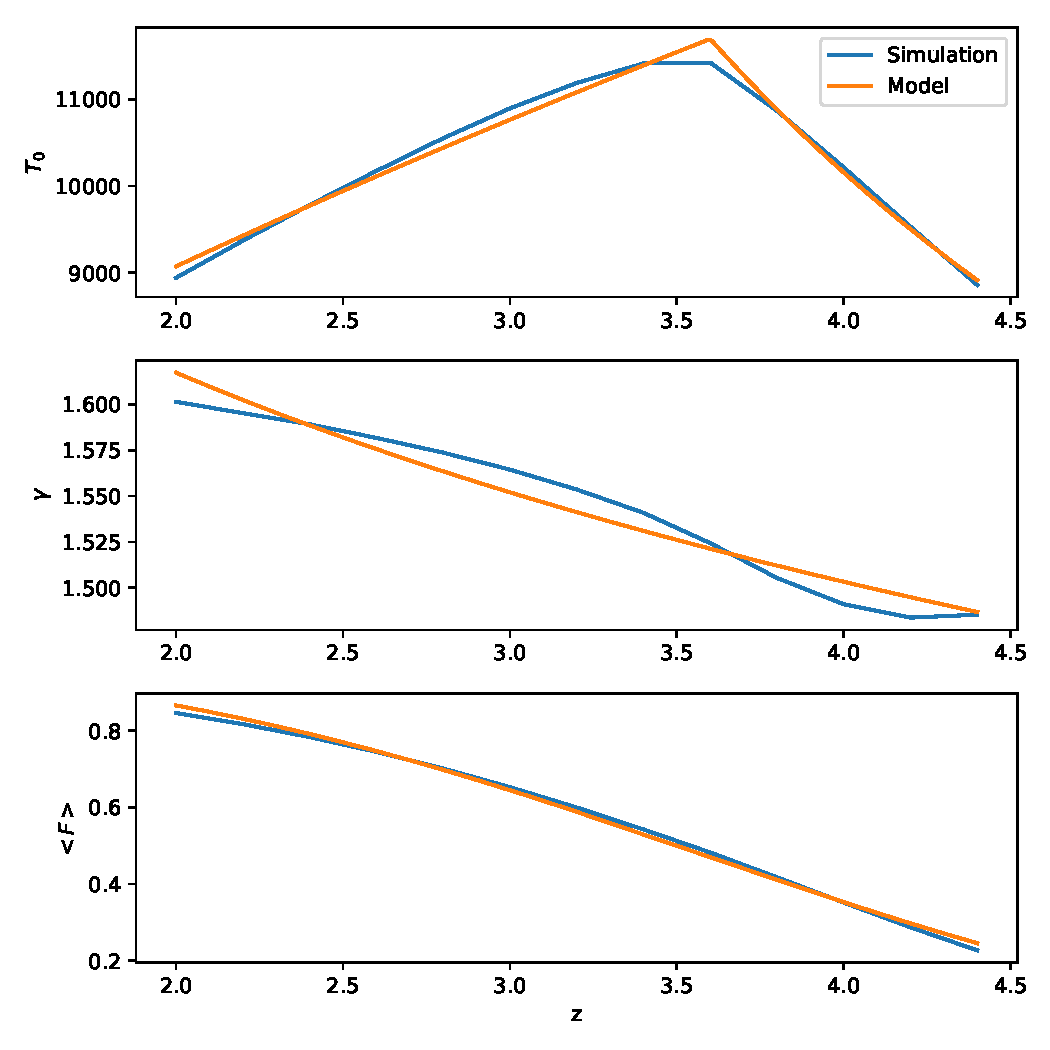
\includegraphics[scale=0.7]{Figures/512_sim2.pdf}
    \caption{The redshift evolution of three of the emulator nuisance parameters for a 
    randomly chosen simulation. In blue we show the measured redshift evolution in the 
    simulation, in orange we show the best fit model using the likelihood models 
    described in section 2.2.}
\end{figure}

\section{Extensions}

\end{document}
